%%\documentclass[a4paper, 12pt]{scrreprt}

\documentclass[a4paper, 12pt]{scrartcl}
%usepackage[german]{babel}
\usepackage{microtype}
%\usepackage{amsmath}
%usepackage{color}
\usepackage[utf8]{inputenc}
\usepackage[T1]{fontenc}
\usepackage{wrapfig}
\usepackage{lipsum}% Dummy-Text
\usepackage{multicol}
\usepackage{alltt}
%%%%%%%%%%%%bis hierhin alle nötigen userpackage
\usepackage{tabularx}
\usepackage[utf8]{inputenc}
\usepackage{amsmath}
\usepackage{amsfonts}
\usepackage{amssymb}

%\usepackage{wrapfig}
\usepackage[ngerman]{babel}
\usepackage[left=25mm,top=25mm,right=25mm,bottom=25mm]{geometry}
%\usepackage{floatrow}
\setlength{\parindent}{0em}
\usepackage[font=footnotesize,labelfont=bf]{caption}
\numberwithin{figure}{section}
\numberwithin{table}{section}
\usepackage{subcaption}
\usepackage{float}
\usepackage{url}
%\usepackage{fancyhdr}
\usepackage{array}
\usepackage{geometry}
%\usepackage[nottoc,numbib]{tocbibind}
\usepackage[pdfpagelabels=true]{hyperref}
\usepackage[font=footnotesize,labelfont=bf]{caption}
\usepackage[T1]{fontenc}
\usepackage {palatino}
%\usepackage[numbers,super]{natbib}
%\usepackage{textcomp}
\usepackage[version=4]{mhchem}
\usepackage{subcaption}
\captionsetup{format=plain}
\usepackage[nomessages]{fp}
\usepackage{siunitx}
\sisetup{exponent-product = \cdot, output-product = \cdot}
\usepackage{hyperref}
\usepackage{longtable}
\newcolumntype{L}[1]{>{\raggedright\arraybackslash}p{#1}} % linksbündig mit Breitenangabe
\newcolumntype{C}[1]{>{\centering\arraybackslash}p{#1}} % zentriert mit Breitenangabe
\newcolumntype{R}[1]{>{\raggedleft\arraybackslash}p{#1}} % rechtsbündig mit Breitenangabe
\usepackage{booktabs}
\renewcommand*{\doublerulesep}{1ex}
\usepackage{graphicx}


\usepackage[backend=bibtex, style=chem-angew, backref=none, backrefstyle=all+]{biblatex}
\bibliography{Literatur.bib}
\defbibheading{head}{\section{Literatur}\label{sec:Lit}} 
\let\cite=\supercite
%\begin{document}
\setlength\abovedisplayshortskip{20pt}
\setlength\belowdisplayshortskip{20pt}
\setlength\abovedisplayskip{20pt}
\setlength\belowdisplayskip{20pt}
\section {Auswertung}
Zur Bestimmung des Diffusionskonstanten wurden die gemessenen relativen Füllstände in ein Längenmaß umgerechnet. Unter Kenntnis der gewählten Entfernung des Miniskus bei Zeitpunkt $t_0$ zur Mitte des Luftdurchströmten Stefanrohrs (vgl. Durchführung), sowie der Relation der verwendeten Skalen mit $1\,[\si{mL}] \sim 2\,[\si{cm}] \Rightarrow \frac{2}{1}\,\left[ \si{\frac{cm}{mL}}\right] $ folgt :\\
\\
Sei $z$ die zu bestimmende Längendifferenz sowie $x_{\Delta}$ die gemessene Füllhöhendifferenz.
\begin{equation}
z(x_{\Delta})= (x_{Mess}-x_{Start}) \cdot 2= x_{\Delta} \cdot 2
\end{equation}
Als Fehler wurde für die Zeitmessung eine gemittelte Ungenauigkeit von $5\,[\si{s}]$ begründet durch Reaktionszeit und Ablesedauer angenommen. Für den ermittelten Füllstand ergibt sich ein konstanter Ablesefehler von $0.005 \,[\si{mL}]$. Der Fehler der errechneten Längendifferenz ergibt sich aus der Fehlerrechnung wie folgt : 
\begin{equation}
	\Delta z = \left|\frac{\partial z(x_{\Delta})}{\partial x_{\Delta}}\right| \cdot \Delta x = 2 \cdot 0.005 = 0.01
\end{equation}
Die nachfolgende Tabelle fasst die Messergebnisse und Längendifferenzen zusammen.
\begin{table}[H]
	\centering
	\label{Messdaten}
	\caption{Messwerte der insgesamt 17 Messungen der Zeitdifferenz ausgehend von $t_0$, dem relativen Füllstandes sowie den errechneten Längendifferenzen. Der Fehler wurde in allen Fällen als konstant und absolut angenommen. Für die Zeit wurde eine Unsicherheit von $5\,[\si{s}]$, für den Füllstand ein Ablesefehler von $0.005 \,[\si{mL}]$ gewählt. Der Fehler der Längendifferenz errechnet sich wie oben.\\}
	\begin{tabular}{C{0.15\linewidth}|C{0.2\linewidth}C{0.2\linewidth}C{0.25\linewidth}}
		Messung  &  Zeitdifferenz $\left[\si{s}\right] $ &  Füllstand $\left[\si{mL}\right] $ & Längendifferenz $[\si{cm}]$\\
		\hline \addlinespace[1ex] 
		$ 1$ & $ 490 $ & $17.425$ & $0.15$\\
		$2$ & $790$& $ 17.450$ &$0.20$\\
		$3$ & $1090$& $17.500$  &$0.30$\\
		$4$ &$1390$& $17.525$ &$0.35$\\
		$5$&  $1690 $&  $17.550$ &$0.4$\\
		$6$&  $1990 $&  $17.575$ &$0.45$\\
		$7$ &  $2290$&$17.600$ &$0.50$\\
		$8$ & $2590 $&$17.625$  &$0.55$\\
		$9$ &  $2890 $& $17.650$  &$0.60$\\
		$10$ &  $3190 $& $17.675$  &$0.65$\\
		$11$ &  $3490 $& $17.70$  &$0.70$\\
		$12$ &  $3790 $& $17.725$  &$0.75$\\
		$13$ &  $4090 $& $17.750$  &$0.80$\\
		$14$ &  $4390 $& $17.775$  &$0.85$\\
		$15$ &  $4690 $& $17.800$  &$0.90$\\
		$16$ &  $4990 $& $17.825$  &$0.95$\\
		$17$ &  $5290 $& $17.850$  &$1.00$\\
		\hline \addlinespace[1ex] 
		absolute &$\Delta t$ &$\Delta x$ &$\Delta z$\\Fehler & $\pm 5$& $\pm 0.005$  & $\pm 0.01$ \\
		
	\end{tabular}
\end{table}
Betrachtet man die Auftragung der ermittelten Längendifferenz über der Zeit ergibt sich ein in guter Näherung linearer Verlauf gemäß :
\begin{figure}[H]
	\centering	
	\begin{minipage}{1\textwidth}
		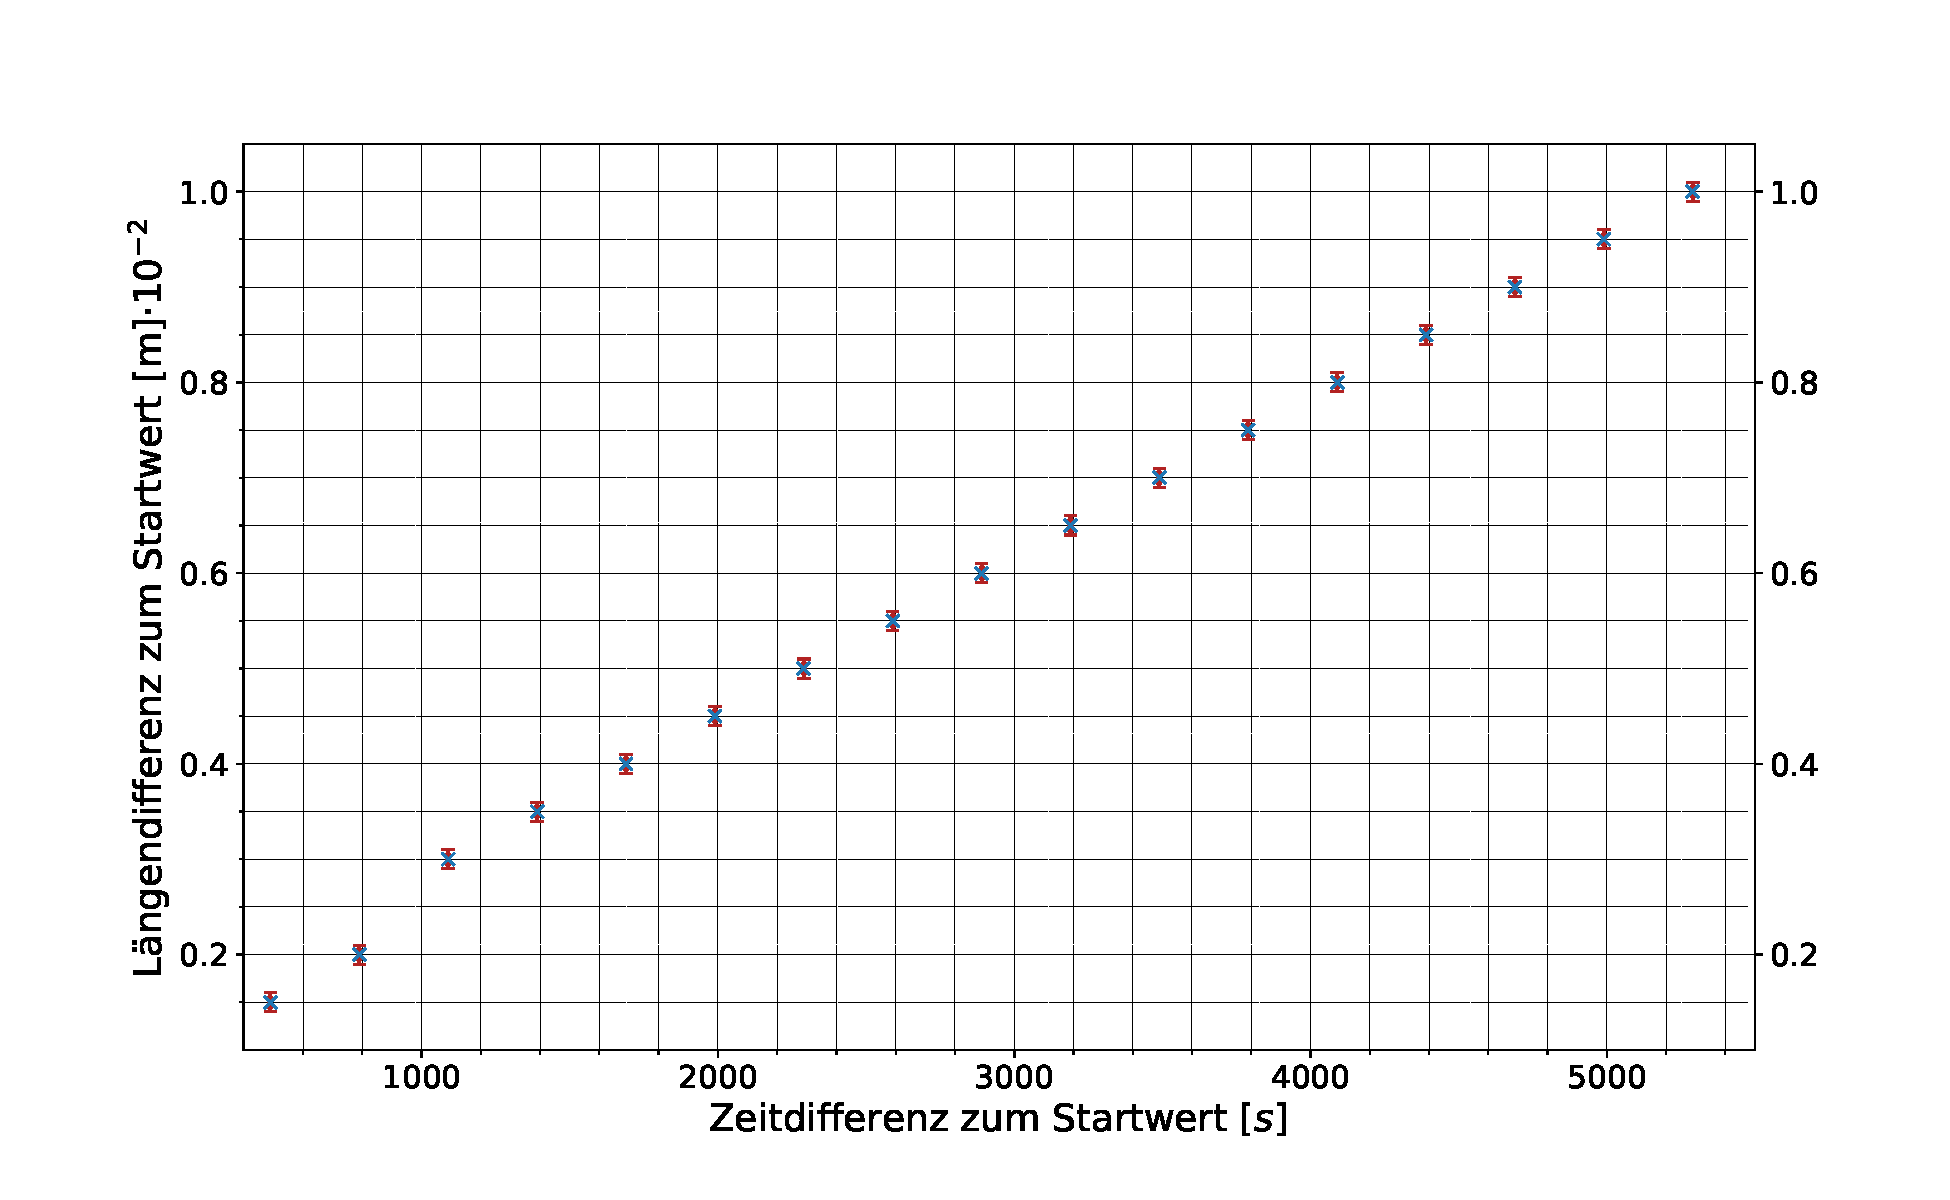
\includegraphics[width=\columnwidth]{Messreihe.pdf}
	\end{minipage}
	\caption{Auftragung der errechneten Längendifferenzen über den gemessenen Zeitdifferenzen durch die Programmierumgebung \textit{python}. Die Messwerte wurden in blau sowie die Fehlerbalken in rot dargestellt.}
	\label{Messreihe}
\end{figure} 
Mit Gleichung \ref{eq:diffkonst} kann durch die folgenden, als konstant und fehlerfrei angenommenen, Werten die Diffusionskonstanten für jedes Wertepaar berechnet werden. Zur Bestimmung des Dampfdrucks wurde die Antoine-Gleichung gemäß des Versuchsskriptes verwendet. 
\begin{equation}
log_{10}(p^D) = A-(\frac{B}{T+C})
\end{equation}
wobei die Parameter $A,B,C$ im Skript zum Experiment gegeben waren, und für $T$ die Arbeitstemperatur gewählt wurde.
\begin{table}[H]
	\centering
	\label{Konstanten}
	\caption{Tabelle der für die Berechnung der Diffusionskonstanten verwendeten, als konstant angenommenen, Größen mit Einheit. \cite{Skript} }
	\begin{tabular}{C{0.4\linewidth}|C{0.2\linewidth}|C{0.2\linewidth}}
		Größe  &  Zahlenwert & SI-Einheit\\
		\hline \addlinespace[1ex] 
		Universelle Gaskonstante  : $R$&  $8.3144598$&$ \left[\si{\frac{kg\cdot m^2}{s^2 \cdot  mol \cdot K}}  \right]$  \\
		Molare Masse Isopentan : $M$ & $72.15\cdot 10^{-3}$ & $\left[ \si{\frac{kg}{mol}}\right]$\\
		Dampfdruck : $p^D$& $95059.21$ & $\left[ \si{\frac{kg}{m \cdot s^2}}\right]$\\
		Arbeitstemperatur : $T$ & $299.16$& $[ \si{K}]$ \\
		Außendruck : $p^0$ & $100430$& $\left[ \si{\frac{kg}{m\cdot s^2}} \right]$ \\
		Dicht Isopentan : $\rho$ & $0.62\cdot 10^3 $& $\left[ \si{\frac{kg}{m^3}}\right]$ \\
	\end{tabular}
\end{table}
Exemplarisch wird hier die einfache Berechnung der Diffusionskonstanten aus dem ersten Wertepaar, sowie dessen Fehler, durchgeführt. Für die weiteren 16 Wertepaare war das Vorgehen analog. Zur Berechnung wird die im theoretischen Teil verwendete Zusammenfassung der Konstanten in einem $K$ übernommen.
\begin{equation}
D_{AB} = -K \cdot \frac{(5.15\cdot 10^{-2} \,\si{m})^2-(5\cdot 10^{-2} \,\si{m})^2}{490\,\si{s}} = 11.3 \cdot 10^{-6} \,[\si{\frac{m^2}{s}}]
\end{equation}
wobei sich der Konstante Faktor $K$ wie folgt errechnet : 
\begin{equation}
K = \frac{8.314 \,\si{\frac{kg\cdot m^2}{s^2 \cdot  mol \cdot K}}\cdot 299.16\,\si{K} \cdot 0.62\cdot 10^3\, \si{\frac{kg}{m\cdot s^2}}}{2\cdot  100430\,\si{\frac{kg}{m\cdot s^2}}\cdot 72.15\cdot 10^{-3}\,\si{\frac{kg}{mol}}}\cdot \left(ln\left(1-\frac{95059.21\,\si{\frac{kg}{m \cdot s^2}}}{100430\,\si{\frac{kg}{m\cdot s^2}}}\right)\right) ^{-1} = -36.34 
\end{equation}
Das diese Konstante einheitenlos ist, kann leicht durch eine Einheiten-Betrachtung begründet werden. Der Gesamtfehler errechnet sich gemäß der partiellen Ableitung nach : 
\begin{equation}
\Delta D_{AB} = \left| \frac{\partial D_{AB}}{\partial z}\right|\cdot \Delta z + \left| \frac{\partial D_{AB}}{\partial z_0}\right|\cdot \Delta z_0 + \left| \frac{\partial D_{AB}}{\partial t}\right|\cdot \Delta t
\end{equation}
Nach Bildung der partiellen Ableitungen resultiert folgende Gleichung, in welche wie bei der Bestimmung von $D_{AB}$ gegebene Wertepaare für $z$ und $t$ eingesetzt werden : 
\begin{equation}
\Delta D_{AB} = -K \cdot \frac{2z}{t} \Delta z + K \cdot \frac{2z_0}{t}\cdot \Delta z_0 -K \cdot \frac{z_0^2-z^2}{t^2}\cdot \Delta t
\end{equation}
\newpage
Es ergeben sich die Diffusionskonstanten mit den absoluten Fehlern wie folgt : 
\begin{table}[H]
	\centering
	\caption{Diffusionskonstanten der 17 gemessenen Wertepaare, berechnet gemäß vorgestellter Beispielrechnung. Die gesamte Berechnung wurde in der Programmiersprache \textit{python} durchgeführt.}
		\label{DiffK}
	\begin{tabular}{C{0.15\linewidth}|C{0.2\linewidth}C{0.3\linewidth}}
		Messung  &  Diffusionskonstante $10^{-6} \,\,\,\left[\si{\frac{m^2}{s}}\right] $ &  absoluter Fehler  $10^{-6} \,\,\,\left[\si{\frac{m^2}{s}}\right] $\\
		\hline \addlinespace[1ex] 
		$ 1$ & $ 11.30 $ & $2.25$ \\
		$2$ & $9.38$& $ 1.82$ \\
		$3$ & $10.30$& $1.96$  \\
		$4$ &$9.47$& $1.79$ \\
		$5$&  $8.95 $&  $1.68$ \\
		$6$&  $8.59 $&  $1.60$ \\
		$7$ &  $8.33$&$1.54$ \\
		$8$ & $8.14 $&$1.50$  \\
		$9$ &  $8.00 $& $1.46$  \\
		$10$ &  $7.86 $& $1.43$ \\
		$11$ &  $7.80 $& $1.41$  \\
		$12$ &  $7.73 $& $1.39$ \\
		$13$ &  $7.68 $& $1.37$  \\
		$14$ &  $7.63 $& $1.36$  \\
		$15$ &  $7.60 $& $1.35$  \\
		$16$ &  $7.58 $& $1.36$  \\
		$17$ &  $7.56 $& $1.33$\\
	\end{tabular}
\end{table}
Es wird das harmonische Mittel der erhaltenen Diffusionskonstanten gemäß folgender Formel ermittelt. Hierfür, und für jede weitere durchgeführte statistische Analyse wurde die Programmiersprache \textit{python} verwendet.
\begin{equation}
\overline{{D_{AB}}}= \frac{\sum D_{AB}}{\# D_{AB}} = 8.47\cdot 10^{-6}\left[ \,\si{\frac{m^2}{s}} \right]
\end{equation}
Der Fehler der gemittelten Diffusionskonstante ergibt sich als harmonisches Mittel der in der Tabelle \ref{DiffK} bestimmten Fehler. Somit also : 
\begin{equation}
\overline{{\Delta D_{AB}}}= \frac{\sum \Delta D_{AB}}{\# \Delta D_{AB}} = 1.58\cdot 10^{-6}\left[ \,\si{\frac{m^2}{s}} \right]
\end{equation}
Um Einschätzung des Streumaßes der durchgeführten Mittelwertbildung zu erhalten kann die Standartabweichung gemäß folgender Gleichung ermittelt werden : 
\begin{equation}
\sigma_{\overline{D_{AB}}} = \frac{\sum (D_{AB}-\overline{D_{AB}})}{\# D_{AB}} = 1.05\cdot 10^{-6}\left[ \,\si{\frac{m^2}{s}} \right]
\end{equation}
%\end{document}